\documentclass[12pt]{article}
\usepackage[a4paper, total={6in, 8in}]{geometry}

%\setlength{\parskip}{3pt}

\usepackage{amsmath}
\usepackage{amssymb}
\usepackage{graphicx}
\usepackage{siunitx}
\usepackage{authblk}
\usepackage{url}

\bibliographystyle{ieeetr}

\begin{document}

\title{Can liquid crystal phases be identified via machine learning?}
\author{Joshua Heaton}
\affil{School of Physics and Astronomy, The University of Manchester\\}
\date{\today}

\maketitle

\begin{abstract}
hi
\end{abstract}

\pagenumbering{gobble}
\newpage
\pagenumbering{arabic}

%=========================================================================================
\section{Introduction}
Machine learning methods have seen widespread utilisation across all scientific disciplines, in situations where conventional algorithms are too cumbersome to implement for specific data-based and modelling tasks \cite{Carleo19}. Deep learning, loosely defined as machine learning with large datasets, parallel computation and scalable algorithms with many layers \cite{Goodfellow16}, has and continues to increase the range and complexity of possible applications of machine learning in the sciences \cite{Carleo19}. Any task applying deep learning to data with a grid-like form, such as images, likely involves the usage of convolutional neural network (CNN) algorithms \cite{Goodfellow16}. CNNs were conceived in 1989 by Yann LeCun et al. and successfully applied to recognition of handwritten characters \cite{LeCun89}. However, their astounding performance in the field of computer vision would not be fully realised until after breakthroughs in deep learning starting in 2006 \cite{Goodfellow16}. Their efficacy was further proven when Geoffrey Hinton \textit{et al.} entered a CNN into the ImageNet Large Scale Visual Recognition Challenge in 2012, and won by a large margin \cite{ILSVRC15}.

Liquid crystal phases are in general identified by eye, directly from textures taken by polarised microscopy. Without adequate experience, this can prove a difficult task because certain unique liquid crystal phases, generated by often minor changes in structural properties, can have similar textural appearances \cite{Dierking03}. Our project aims to test the viability of machine learning algorithms as tools to assist phase identification. CNNs are particularly suitable due to their prevalence in image classification, and so form the core of our investigations. Current literature in this specific topic is limited, and the approaches so far have mostly involved the usage of simulated textures in the training of models \cite{Sigaki20, Minor20}. Sigaki et al. have demonstrated the viability of CNNs in isotropic and nematic phase texture classification and in the prediction of physical liquid crystal properties \cite{Sigaki20}. Our study further explores and attempts to push the limits of the classification task across a wider range of phases, utilising real experimental data produced by polarised microscopy.

This project report will first provide a brief overview of the physics behind liquid crystals and the capturing of their textures by polarised microscopy, as well as an introduction to machine learning, neural networks and CNNs. The details and results of our investigations into phase classification will then be presented, as well as an outlook to further study.
%=========================================================================================
\section{Liquid crystal phases}
Liquid crystals are substances in a state between that of a fully isotropic liquid and a crystal with a periodic lattice structure. The molecules can have varying positional order, and have orientational order over large sections. The unit vector parallel to the alignment of the molecules is called the director. Other details such as molecular shape and chirality affect the overall structure. These variations in structure result in numerous individual identifiable liquid crystal phases. Thermotropic liquid crystals exhibit phases transitions with changing temperature, whereas lyotropic liquid crystals are dissolved in a solvent with the phase depending on the concentration \cite{Demus99}. This project will be concerned with only thermotropic liquid crystals. 

When cooling a thermotropic liquid crystal starting as an isotropic liquid, it will first transition to the nematic phase (N), which has orientational order only. The chiral nematic (cholesteric, N*), phase also has no positional order, and has a periodic variation of the director, resulting in helical structures. Upon further cooling, the smectic phase will be reached. This can be split into three categories, going from fluid smectic to hexatic smectic to soft crystal in order of decreasing temperature. The fluid smectic phase has molecules arranged in layers, with no positional order in the plane of each layer. When the director is perpendicular to the layer planes, the phase is smectic A (SmA), with smectic C (SmC) having a director that is tilted by comparison. Hexatic smectic phases have short range positional order within the layer planes with hexagonal intermolecular arrangements interspersed with order-breaking defects. This encompasses the smectic B (SmB), I (SmI), and F (SmF) phases. Semctic B has a director perpendicular to the layer planes, whereas it is tilted towards the vertices of the hexagons for smectic I and towards to the sides of the hexagons for smectic F. The soft crystal phases are defect free within the layers and therefore exhibit long range positional order \cite{Dierking03}.

The liquid crystal texture data used in this project have all been obtained by polarised microscopy captured with a video camera. In brief terms, a polarising microscope works by placing a sample between perpendicularly aligned polarisers. When light is shone through the arrangement the resulting image will be dark, unless the sample rotates the plane of polarisation. In the case of liquid crystals, the isotropic liquid phase has no optical properties so will produce completely dark textures. The nematic, cholesteric and smectic phases are anisotropic and therefore birefringent, with optical axes depending on their structures. This produces unique textural image features for each phase \cite{Dierking03}. Some example textures taken from our dataset are displayed in Figure 1.

\begin{figure}[h]
\centering
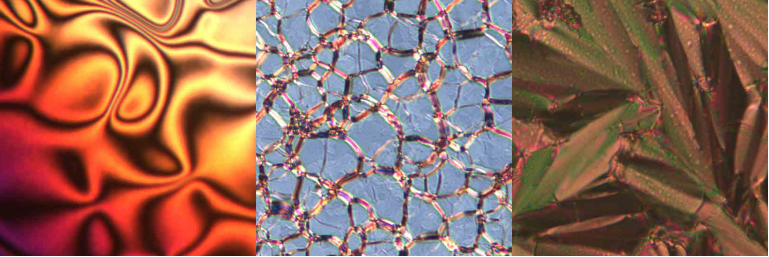
\includegraphics[width=6in]{images/texture_samples.png}
\caption{Liquid crystal textures from the dataset, from left to right: nematic phase compound 5CB, cholesteric phase compound D5, and smectic C phase compound M10.}
\end{figure}
%=========================================================================================
\section{General machine learning principles}
A machine learning model is a computer algorithm which automatically improves its performance in a given task as it gains experience from a dataset \cite{Goodfellow16}. It learns patterns in data and uses these patterns to make probabilistic predictions. The data normally takes the form of a set of $N$ examples, which are usually expressed as vectors, or some other structure of features, $\{\mathbf{x}_i\}_{i=1}^N$, containing quantitative information about example $i$. In supervised learning the examples are given labels $y_i$, to form a training set of inputs and outputs $\{\mathbf{x}_i, y_i\}_{i=1}^N$, and the model attempts to learn the mapping from a general input $\mathbf{x}$ to an output $y$. One main type of supervised learning is regression, in which the output is a numerical scalar. The other main type is classification, in which the model produces a normalised vector of probabilities corresponding to categories. The output of the model is taken as the category with the highest probability. In unsupervised learning there are no labels, and the algorithm attempts to learn specific patterns in the dataset such as clusters of similar data points \cite{Murphy12}. The topic of this project is a supervised classification problem.

From now on the labels on a training set will be denoted as $y^{(\textrm{true})}$, and the outputs of a model as $y^{(\textrm{pred})}$. A supervised model can be expressed as a function of inputs and a set of parameters $\{\theta\}$ such that $y^{(\textrm{pred})}=f(\mathbf{x},\{\theta\})$. Training involves optimisation of the parameters by minimisation of a cost function $J(y^{(true)},y^{(pred)})$, which measures the deviation of the predictions of the model from the true labels. The most common optimisation algorithms involve computing the gradient of $J$ with respect to $\{\theta\}$ \cite{Goodfellow16}. 

The capacity of a model is akin to its complexity. The number of trainable parameters can give a fast indication of capacity. However, it also depends on the model's functional form. The parameters controlling the capacity of the model, as well as certain other training settings, are known as hyperparameters. If the capacity is too small, the model will tend to "underfit" the training set, resulting in poor performance even when optimised well. On the other hand, too high a capacity will result in "overfitting", with high performance on the training set, but the model may not generalise well to new unseen data. Methods for reducing overfitting are known as regularisation. Before training begins, the entire dataset is often split into training, validation, and test sets, denoted as $\mathbf{x}^{(\textrm{train})}$, $\mathbf{x}^{(\textrm{valid})}$ and $\mathbf{x}^{(\textrm{test})}$ respectively. The training set, as defined previously, is used to optimise the parameters. The model's performance is then evaluated on the validation set. A poor performance on both the training and validation sets is indicative of underfitting, whereas a high performance on the training set and low on the validation set suggests overfitting. The validation set can therefore be used to tune the hyperparameters of the model before retraining. This can be repeated until the model fits optimally. The final model is then evaluated on the as-of-yet unseen test set to determine its overall efficacy \cite{Goodfellow16}.
%=========================================================================================
\section{Neural networks}
a
\subsection{Hidden units and network architecture}
a
\subsection{Neural network training}
a
\subsection{Regularisation methods}
a
%=========================================================================================
\section{Convolutional neural networks}
a
\subsection{Convolutional layers}
a
\subsection{Pooling layers}
a
%=========================================================================================
\section{4-phase classifier models}
a
\subsection{Dataset preparation}
a
\subsection{Model architectures and training configuration}
a
\subsection{Results}
a
%=========================================================================================
\section{Smectic phase classifier models}
a
\subsection{Dataset preparation}
a
\subsection{Model architectures and training configuration}
a
\subsection{Results}
a
%=========================================================================================
\section{Smectic A and C binary classifier models}
a
\subsection{Dataset preparation}
a
\subsection{Model architectures and training configuration}
a
\subsection{Results}
a
%=========================================================================================
\section{Conclusions}
a
%=========================================================================================
\section{Going forward}
a
%=========================================================================================

\bibliography{report}

\end{document}